\chapter{5. Observer Pattern}

\section{Giới thiệu}
\subsection{Đặt vấn đề}
Chúng ta cần thiết kế và xây dựng một hệ thống phần mềm cho một trạm quan sát thời tiết. Dữ liệu của hệ thống được xây dựng thông qua một đối tượng gọi là WeatherData - đóng vai trò theo dõi điều kiện thời tiết hiện tại (nhiệt độ, độ ẩm, áp suất).\\
Yêu cầu ứng dụng cung cấp 3 phần tử màn hình hiển thị:
\begin{itemize}
    \item CurrentConditionDisplay
    \item StatsisticsDisplay
    \item ForcastDisplay
\end{itemize}
Tất cả sẽ được cập nhật theo thời gian thực mỗi khi đối tượng WeatherData lấy được dữ liệu mới nhất.\\
Ngoài ra, trạm quan sát cũng muốn "public" những API để những lập trình viên khác có thể viết ra những màn hình hiển thị thời tiết của riêng họ.\\
Trong trường hợp trên, để có một thiết kế tốt có nghĩa là tách rời càng nhiều càng tốt và giảm sự phụ thuộc. Mẫu thiết kế Observer (quan sát) có thể được sử dụng bất cứ khi nào mà một đối tượng có sự thay đổi trạng thái, tất các thành phần phụ thuộc của nó sẽ được thông báo và cập nhật một cách tự động.
\subsection{Mục đích sử dụng}
Observer Pattern phục vụ mục đích:
\begin{itemize}
    \item Thường được sử dụng trong mối quan hệ 1-n giữa các đối tượng với nhau. Trong đó một đối tượng thay đổi và muốn thông báo cho tất cả các đối tượng liên quan biết về sự thay đổi đó.
    \item Cần đảm bảo rằng khi một đối tượng thay đổi trạng thái, một số đối tượng phụ thuộc kết thúc mở sẽ được cập nhật tự động.
    \item Có thể một đối tượng có thể thông báo cho một số đối tượng khác kết thúc mở.
    
\end{itemize}
Việc xác định phụ thuộc một-nhiều giữa các đối tượng bằng cách xác định một đối tượng (chủ thể) cập nhật trạng thái của các đối tượng phụ thuộc một cách trực tiếp là không linh hoạt vì nó kết hợp chủ thể với các đối tượng phụ thuộc cụ thể. Tuy nhiên, nó có thể có ý nghĩa từ quan điểm hiệu suất hoặc nếu việc triển khai đối tượng được kết hợp chặt chẽ (hãy nghĩ đến các cấu trúc nhân cấp thấp thực thi hàng nghìn lần một giây). Các đối tượng được kết hợp chặt chẽ có thể khó triển khai trong một số trường hợp và khó sử dụng lại vì chúng tham chiếu và biết về (và cách cập nhật) nhiều đối tượng khác nhau với các giao diện khác nhau. Trong các tình huống khác, các đối tượng được kết hợp chặt chẽ có thể là một lựa chọn tốt hơn vì trình biên dịch sẽ có thể phát hiện lỗi tại thời điểm biên dịch và tối ưu hóa mã ở cấp lệnh CPU.
 
\section{Định nghĩa và mô hình cấu trúc}
\subsection{Định nghĩa}
Observer Pattern là một Design Pattern thuộc nhóm hành vi (Behavioral).Nó xác định sự phụ thuộc một-nhiều giữa một tập hợp các đối tượng, chẳng hạn như rằng khi một đối tượng thay đổi, tất cả những phụ thuộc của nó (observers) đều được thông báo và được cập nhật tự động.
\subsection{Mô hình cấu trúc}
\begin{figure}[!htb]
    \centering
    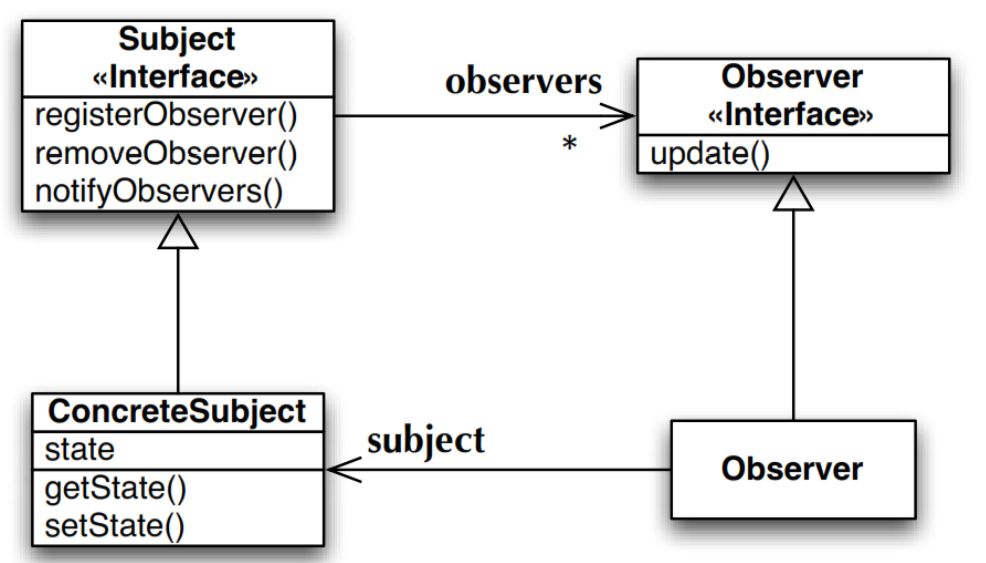
\includegraphics[width=\textwidth]{fig/Observer/structure_observer.png}
    \caption{Mô hình cấu trúc Observer Pattern}
    \label{fig:structure_observer}
\end{figure}
\begin{itemize}
     \item Subject : chứa danh sách các observer,  cung cấp phương thức để có thể thêm và loại bỏ observer.
    \item Observer : định nghĩa một phương thức update() cho các đối tượng sẽ được subject thông báo đến khi có sự thay đổi trạng thái.
    \item ConcreteSubject : cài đặt các phương thức của Subject, lưu trữ trạng thái danh sách các ConcreateObserver, gửi thông báo đến các observer của nó khi có sự thay đổi trạng thái.
    \item ConcreteObserver : cài đặt các phương thức của Observer, lưu trữ trạng thái của subject, thực thi việc cập nhật để giữ cho trạng thái đồng nhất với subject gửi thông báo đến.
\end{itemize}

\section{Cách cài đặt}
\subsection{Cài đặt chung}
Observer tạo ra sự tương tác được kết hợp lỏng lẻo giữa chủ thể và người quan sát
\begin{itemize}
    \item Điều này có nghĩa là họ có thể tương tác với rất ít kiến thức về nhau
\end{itemize} 
Chú ý
\begin{itemize}
    \item Đối tượng chỉ biết rằng Observer thực hiện giao diện Observer interface.
    \begin{itemize}
        \item Chúng ta có thể thêm / bớt Observer thuộc bất kỳ loại nào bất kỳ lúc nào.
        \item Chúng ta không bao giờ phải sửa đổi đối tượng để thêm một loại Observer mới.
    \end{itemize}
    \item Chúng ta có thể sử dụng lại đối tượng và Observer trong các trường hợp khác.
    \begin{itemize}
        \item Giao diện plug-and-play ở bất kỳ nơi nào Observer được sử dụng.
    \end{itemize}
    \item Observer có thể phải biết về lớp ConcreteSubject nếu nó cung cấp nhiều phương thức liên quan đến trạng thái khác nhau.
    \begin{itemize}
        \item Mặt khác, dữ liệu có thể được chuyển cho Observer thông qua phương thức update().
    \end{itemize}
\end{itemize}

Dưới đây là code minh họa cài đặt Observer Pattern.

\begin{figure}[!htb]
    \centering
    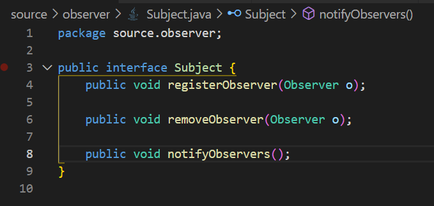
\includegraphics[width=\textwidth]{fig/Observer/subject_class.png}
    \caption{Subject Interface}
    \label{fig:subject_class}
\end{figure}
\begin{figure}[!htb]
    \centering
    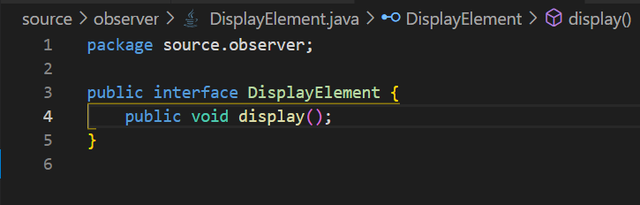
\includegraphics[width=\textwidth]{fig/Observer/display_element_class.png}
    \caption{Display Element Interface}
    \label{fig:display_element_class}
\end{figure}
\newpage
\begin{figure}[!htb]
    \centering
    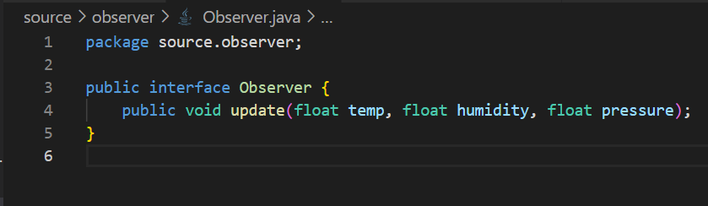
\includegraphics[width=\textwidth]{fig/Observer/observer_class.png}
    \caption{Observer Interface}
    \label{fig:observer_class}
\end{figure}


\subsection{Cài đặt cho một bài toán cụ thể}
Trong bài toán đưa ra ở trên , ta có thể thấy rằng mối quan hệ 1-n ở đây đó là 1-WeatherData và n-Screen . Mỗi khi WeatherData có sự thay đổi về trạng thái (nhiệt độ, độ ẩm, áp suất) thì nó sẽ "thông báo" cho các màn hình đang "quan sát" sát nó để cập nhật lại việc hiển thị thông tin.\\
Do đó chúng ta có Subject ở đây là WeatherData, Observer là các màn hình hiển thị.\\
Mỗi màn hình hiển thị có thể khác nhau, vì thể cách tốt nhất là chúng ta tạo ra một interface cho việc hiển thị.\\
Code minh họa cho bài toán thực tế.\\
Link code cài đặt:
\url{https://github.com/nanhus/OOP-DesginPatten/tree/master/source/observer}
\newpage
\begin{figure}[!htb]
    \centering
    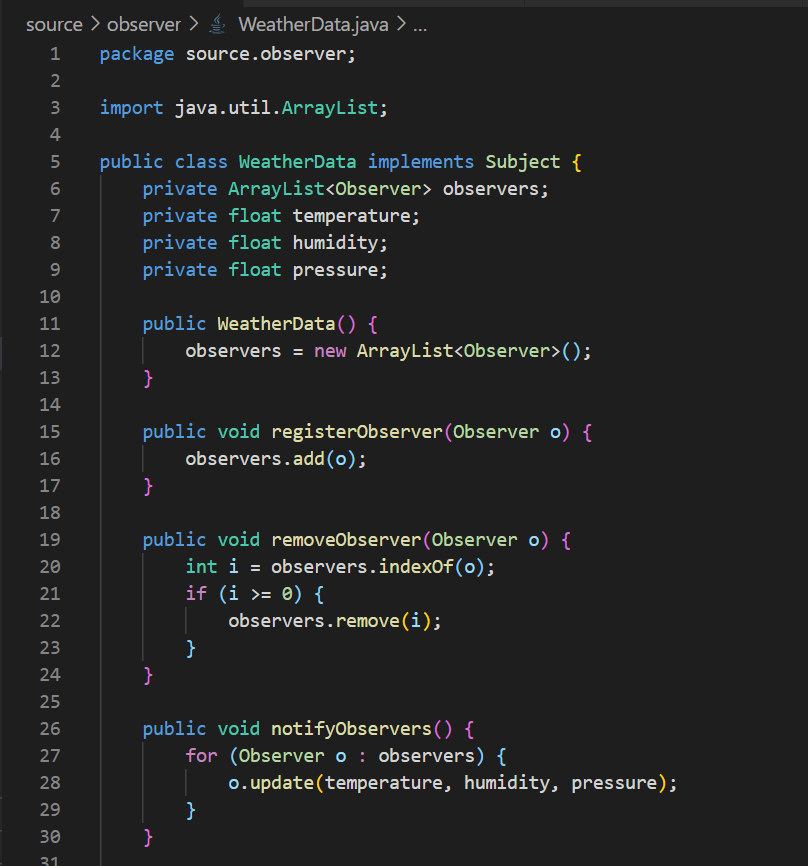
\includegraphics[width=\textwidth]{fig/Observer/weather_data_class.png}
    \caption{Weather Data Class}
    \label{fig:weather_data_class}
\end{figure}
\newpage
\begin{figure}[!htb]
    \centering
    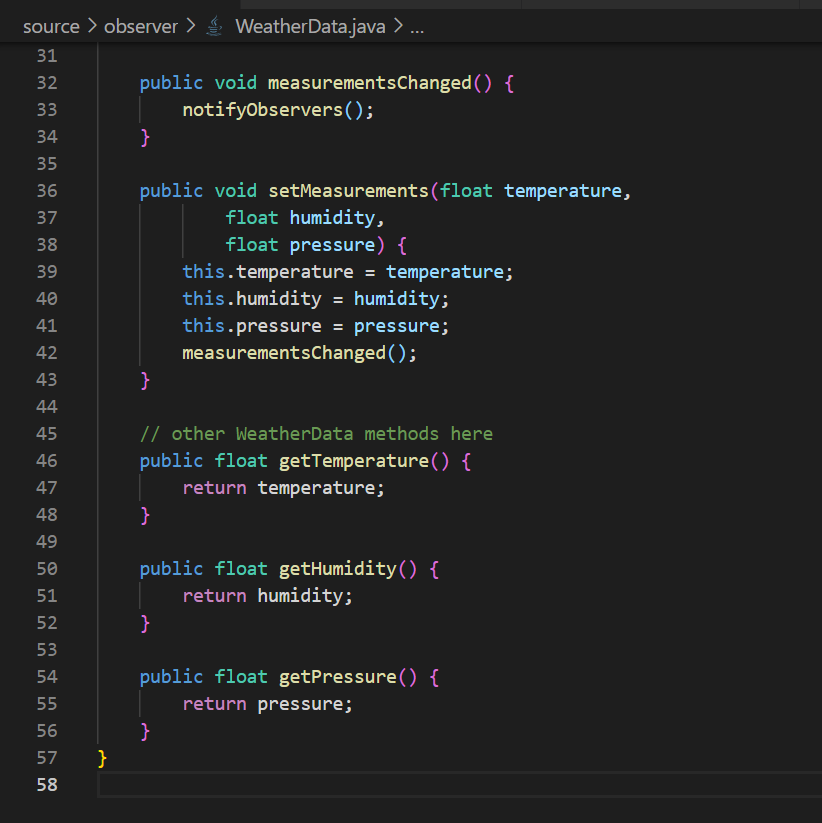
\includegraphics[width=\textwidth]{fig/Observer/weather_data_class_continue.png}
    \caption{Weather Data Class(continue)}
    \label{fig:weather_data_class_continue}
\end{figure}
\newpage
\begin{figure}[!htb]
    \centering
    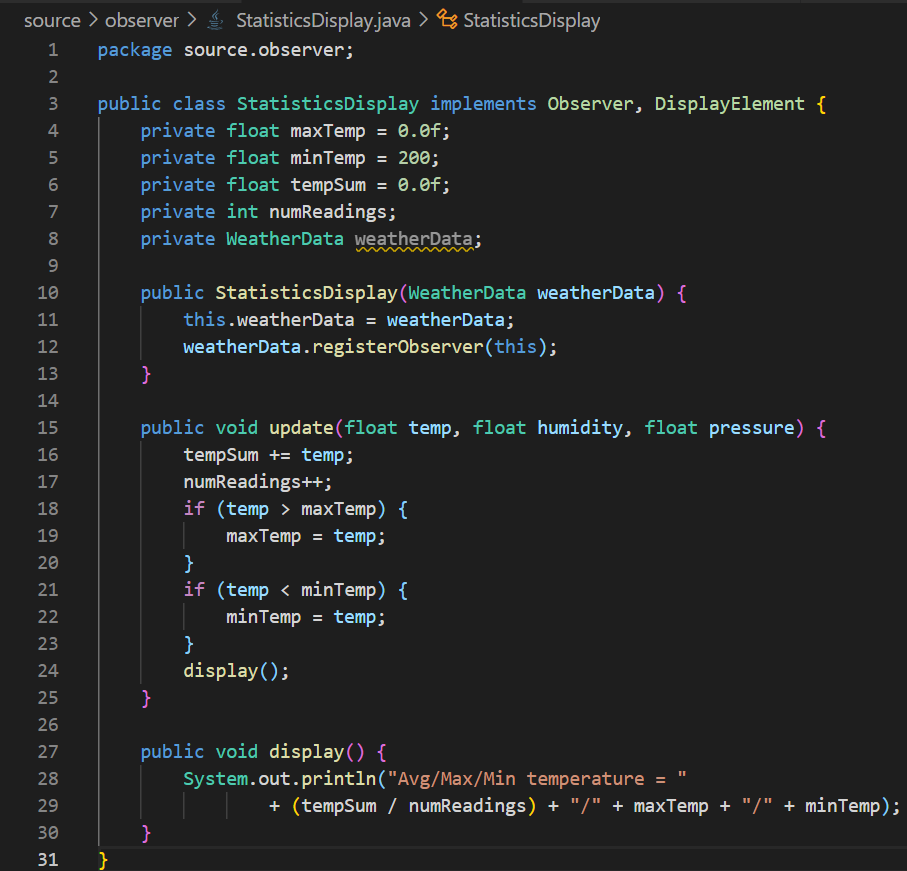
\includegraphics[width=\textwidth]{fig/Observer/statistics_display_class.png}
    \caption{Statistics Display Class}
    \label{fig:statistics_display_class}
\end{figure}
\newpage
\begin{figure}[!htb]
    \centering
    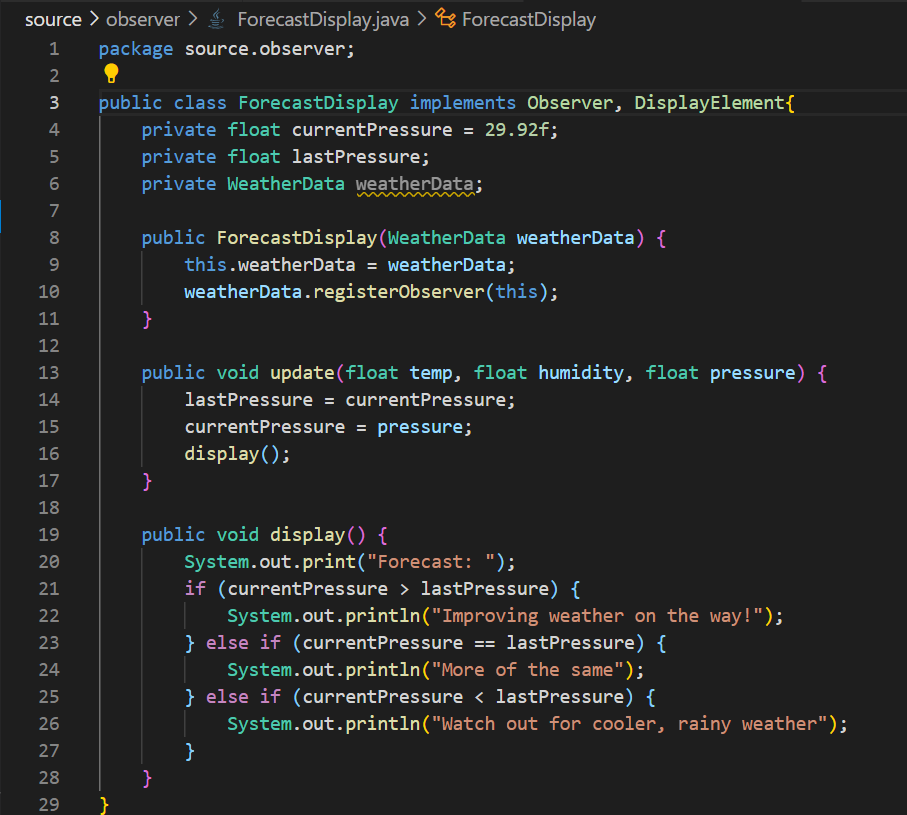
\includegraphics[width=\textwidth]{fig/Observer/forecast_display_class.png}
    \caption{Forecast Display Class}
    \label{fig:forecast_display_class}
\end{figure}
\newpage
\begin{figure}[!htb]
    \centering
    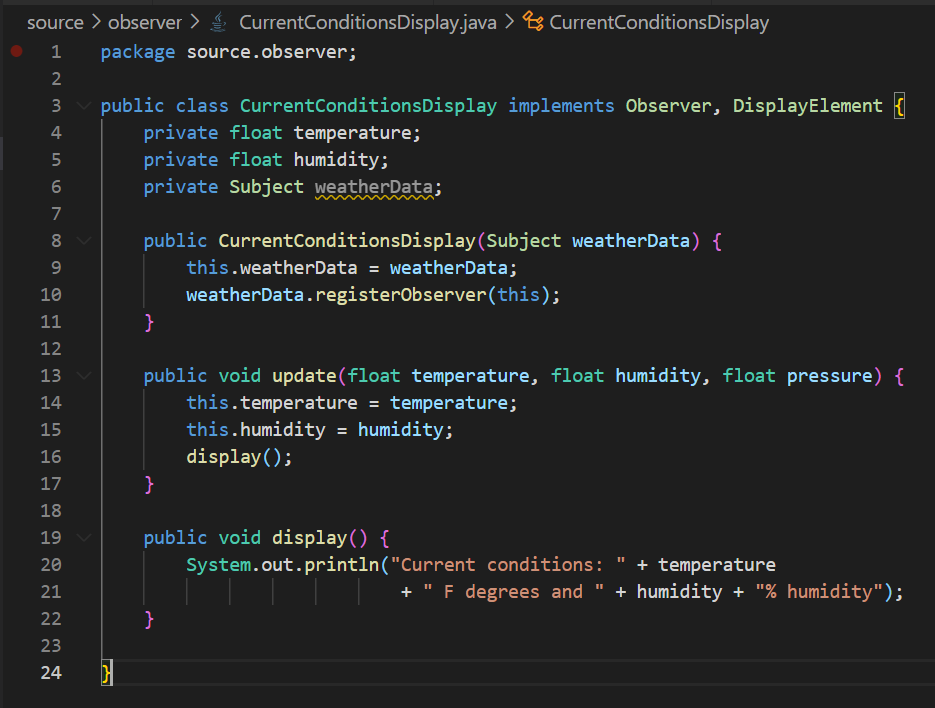
\includegraphics[width=\textwidth]{fig/Observer/current_conditions_display_class.png}
    \caption{Current Conditions Display Class}
    \label{fig:current_conditions_display_class}
\end{figure}
\begin{figure}[!htb]
    \centering
    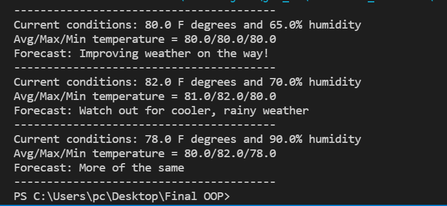
\includegraphics[width=\textwidth]{fig/Observer/observer_output.png}
    \caption{Output}
    \label{fig:observer_output}
\end{figure}

\section{Ví dụ thực tế}
\begin{itemize}
    \item Sử dụng trong ứng dụng broadcast-type communication.
    \item Sử dụng để quản lý sự kiện (Event management).
    \item Sử dụng trong mẫu mô hình MVC (Model View Controller Pattern) : trong MVC, mẫu này được sử dụng để tách Model khỏi View. View đại diện cho Observer và Model là đối tượng Observable.
\end{itemize}
 




